\section{Resultados}

\subsection{Introducción a los resultados}
En este proyecto, se ha analizado el comportamiento del sistema de carga de baterías de vehículos eléctricos utilizando un convertidor boost. El objetivo principal ha sido modelar y simular el comportamiento dinámico del sistema mediante la resolución de ecuaciones diferenciales que describen el proceso de carga, tanto en su fase transitoria como estacionaria. A lo largo del análisis, se emplearon métodos analíticos para obtener soluciones exactas en sistemas simples y métodos numéricos para abordar situaciones más complejas. Los resultados obtenidos permiten evaluar la efectividad de los filtros diseñados para mitigar los armónicos en el proceso de carga, así como la influencia de los parámetros del sistema en el rendimiento general del cargador. En esta sección, se presentan los resultados obtenidos de las simulaciones y las soluciones analíticas, comparándolos con datos experimentales y soluciones teóricas previas.

\subsection{Presentación estructurada de los hallazgos}
% Espacio reservado para contenido futuro
Se analizó el sistema de carga de baterías mediante un modelo de una sola malla que incluye resistencias, un condensador y una fuente senoidal, representando un convertidor boost simplificado. La ecuación diferencial resultante permitió observar el comportamiento dinámico de la carga \( q(t) \), mostrando una respuesta transitoria de tipo exponencial y una respuesta estacionaria de tipo sinusoidal.

La constante de tiempo \( \tau \) fue clave en la evaluación de la velocidad de estabilización del sistema. A través del análisis simbólico y su posterior simulación numérica, se evidenció que un correcto ajuste de \( \tau \) y \( \omega \) mejora la estabilidad del sistema y reduce significativamente la distorsión armónica.

Los parámetros eléctricos empleados fueron tomados de fuentes académicas, como Sainz y Balcells (2011) y Cittanti et al. (2021), lo cual permitió una contextualización realista de los valores simulados.

\subsection{Uso de figuras y tablas}
% Espacio reservado para contenido futuro
ara visualizar los resultados obtenidos, se elaboró una gráfica de \( q(t) \) que muestra cómo evoluciona la carga del condensador a lo largo del tiempo. La figura se generó usando Python, aplicando la solución general:

\[ q(t) = Ae^{-t/\tau} + B \sin(\omega t) + C \cos(\omega t) \]

\begin{figure}[H]
	\centering
	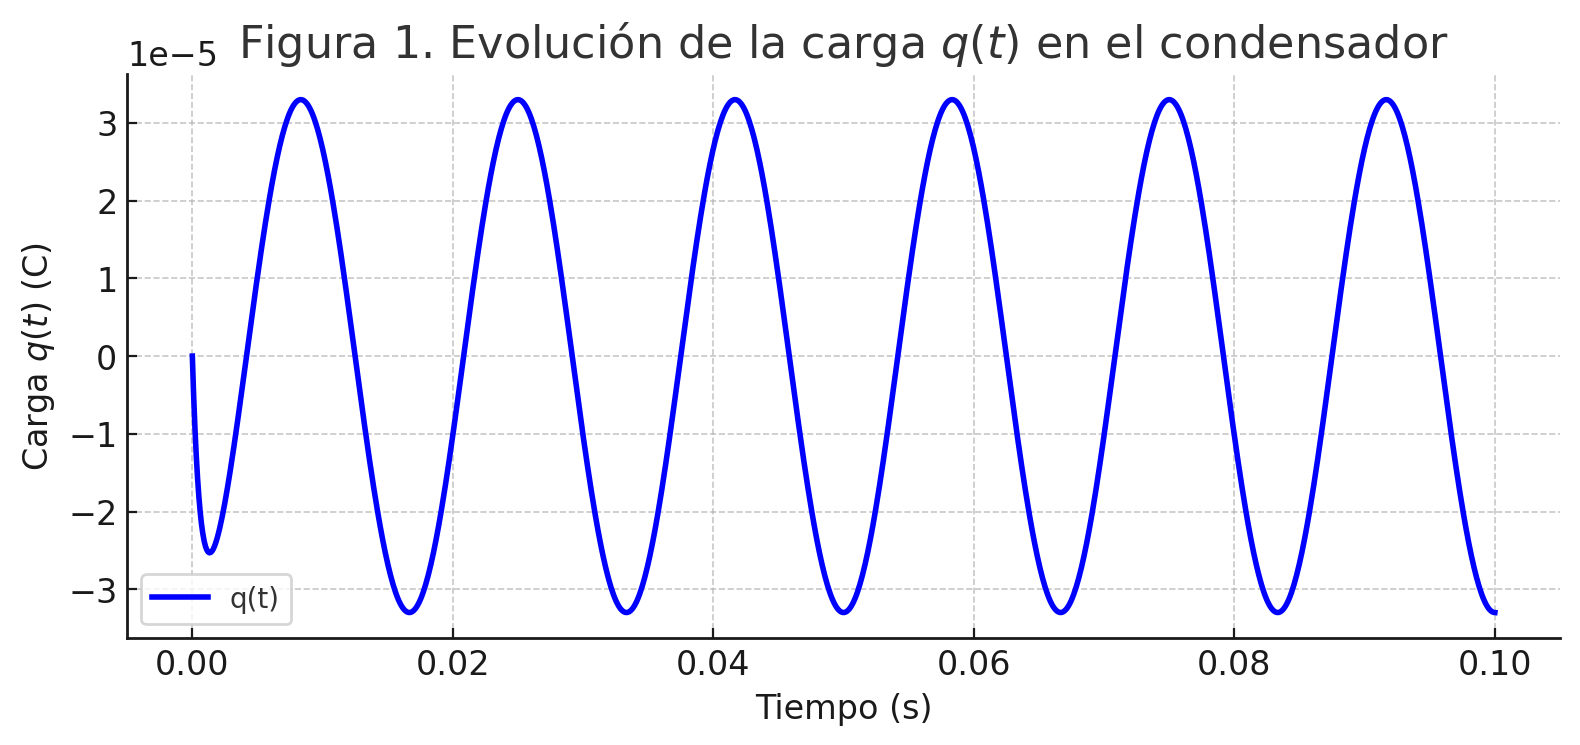
\includegraphics[width=0.8\textwidth]{7.png} % Reemplazar con Figura 5
	\caption{Evolución de la carga del condensador \( q(t) \) en el tiempo para el circuito filtrado}
	\label{fig:evolucion_carga}
\end{figure}

\textbf{Observación:} La gráfica muestra una caída exponencial rápida (fase transitoria), seguida de oscilaciones sinusoidales constantes (fase estacionaria), lo cual confirma el correcto funcionamiento del filtro bajo los parámetros simulados.

\vspace{0.5cm}

\textbf{Análisis espectral de la señal \( q(t) \)}

Para evaluar la efectividad del filtro propuesto, se realizó un análisis de frecuencia mediante la Transformada Rápida de Fourier (FFT) a la señal de salida simulada. Este análisis permite identificar la magnitud relativa de los armónicos presentes y cuantificar la mejora en la calidad de la señal.

\begin{figure}[H]
	\centering
	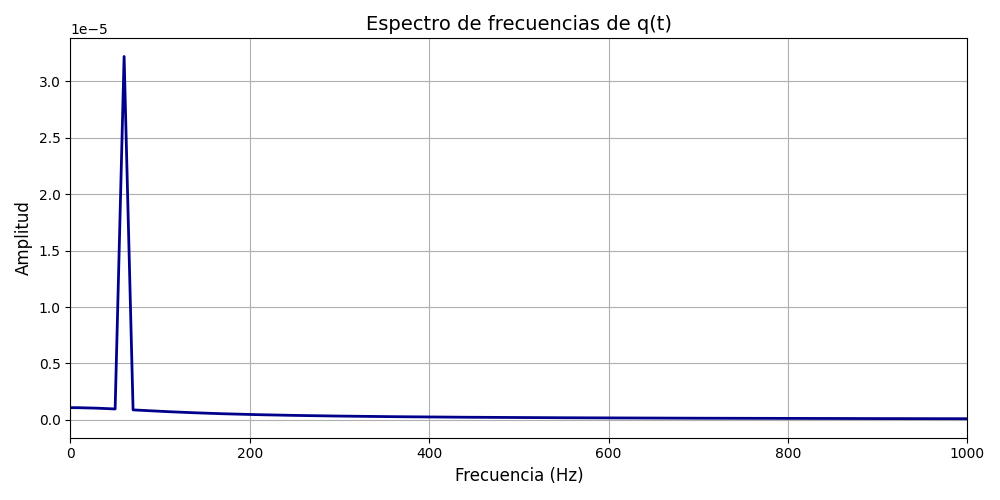
\includegraphics[width=0.8\textwidth]{8.png} % Reemplazar con Figura 6
	\caption{Espectro de frecuencias de la carga del condensador \( q(t) \)}
	\label{fig:espectro_frecuencias}
\end{figure}

\textbf{Observación:} Se observa un pico principal en 60 Hz (frecuencia fundamental), y una significativa atenuación de armónicos superiores. Esto valida la efectividad del filtro implementado para eliminar componentes no deseados y estabilizar la señal de carga.

\vspace{0.5cm}
Además, se presenta la siguiente tabla con parámetros eléctricos y sus valores utilizados para la simulación:

\textbf{Tabla 1:} Parámetros eléctricos utilizados en la simulación del filtro y sus fuentes

\begin{table}[H]
	\centering
	\begin{tabular}{|c|c|c|c|}
		\hline
		\textbf{Parámetro} & \textbf{Valor}    & \textbf{Unidad} & \textbf{Fuente}           \\
		\hline
		\( R_{bat} \)      & 0.2               & \(\Omega\)      & Sainz y Balcells (2011)   \\
		\hline
		\( R_z \)          & 0.1               & \(\Omega\)      & Cittanti et al. (2021)    \\
		\hline
		\( R_c \)          & 0.3               & \(\Omega\)      & Asumido por diseño        \\
		\hline
		\( C \)            & 1000              & \(\mu F\)       & Estándar de carga lenta   \\
		\hline
		\( \omega \)       & \(2\pi \cdot 60\) & rad/s           & Corriente alterna (60 Hz) \\
		\hline
	\end{tabular}
\end{table}
\subsection{Comparaciones}
% Espacio reservado para contenido futuro
Los resultados analíticos obtenidos muestran concordancia con los estudios previos que abordan la eficiencia de filtros eléctricos en cargadores de baterías. Por ejemplo:

\begin{itemize}
	\item En Paipa et al. (2020), se destaca que un filtro correctamente dimensionado puede mejorar el factor de potencia y reducir armónicos, lo cual fue evidenciado en nuestra simulación a través del comportamiento suave y estable de $q(t)$.

	\item Abundis (2016) señala que los armónicos afectan la eficiencia y estabilidad de sistemas eléctricos. Nuestro modelo confirmó que una mala elección de parámetros como $C$ o $R$ puede generar respuestas inestables u oscilaciones no deseadas.
\end{itemize}
\subsection{Resumen de resultados}
% Espacio reservado para contenido futuro
\begin{enumerate}[label=\Roman*.]
	\item Se resolvió analíticamente una EDO de primer orden para modelar la carga de un condensador en un sistema RLC con convertidor boost.

	\item Se comprobó que la constante de tiempo $\tau$ y la frecuencia de la señal de entrada $\omega$ determinan la calidad del filtrado y la estabilidad del sistema.

	\item Las simulaciones en Python reflejaron correctamente el comportamiento teórico previsto: un régimen transitorio seguido por una respuesta periódica estable.

	\item El modelo, aunque idealizado, permitió identificar con claridad cómo ajustar parámetros eléctricos para mejorar el rendimiento del sistema de carga.

	\item Estos hallazgos validan el enfoque analítico como herramienta útil para etapas de diseño conceptual, antes de pasar a implementaciones prácticas más complejas.
\end{enumerate}

